\documentclass{foi}
\usepackage{lipsum}
\usepackage[utf8]{inputenc}
\usepackage{float}

\lstset{basicstyle=\ttfamily,
  showstringspaces=false,
  commentstyle=\color{red},
  keywordstyle=\color{blue},
}

\vrstaRada{\zavrsni}
\title{Izrada aplikacije za pronalazak termina sastanaka}

\author{Leo Ćavar}
\spolStudenta{\musko}
\mentor{Ime Profesora}
\spolMentora{\musko}
\godina{2024}
\mjesec{Rujan}
\date{2024}
\status{redoviti}
\indeks{0016153823}
\smjer{Informacijski i poslovni sustavi}
\titulaProfesora{Doc. Dr. sc.}

\sazetak{Sazetak}

\kljucneRijeci{Kljucno. Kljucno; Kljucno;}

\begin{document}

\maketitle

\tableofcontents

\pagestyle{plain}

\chapter{Uvod}
Primjer poglavlja\cite{API}
\newpage
Primjer popisa\cite{Tyler2024}
\begin{itemize}
    \item U \textit{Google Cloud Console}, potrebno je otići na \textit{IAM \& Admin} te odabrati opciju \textit{Create a Project}.
    \item U polju \textit{Project Name}, unosi se opisni naziv projekta koji jasno definira njegovu svrhu.
    \item Po potrebi, moguće je urediti \textit{Project ID}, no taj ID se ne može mijenjati nakon kreiranja projekta.
    \item Nakon postavljanja imena i ID-a, odabire se lokacija projekta klikom na opciju \textit{Browse} te odabirom odgovarajuće lokacije.
    \item Klikom na \textit{Create}, projekt se kreira unutar nekoliko minuta, a korisnik se preusmjerava na \textit{Dashboard} stranicu unutar \textit{Google Cloud Console}-a.
\end{itemize}

\newpage

\begin{figure}[H]
    \centering
    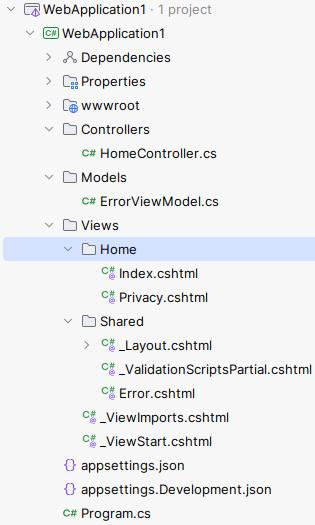
\includegraphics[width=0.2\textwidth]{slike/MVC_project.jpeg}
    \caption{Primjer slike (Izvor: autor)}
    \label{fig:mvc_projekt}
\end{figure}


\chapter{Zaključak}

Zakljucak ide ovdje
\printbibliography[title=Popis literature]
\addcontentsline{toc}{chapter}{Popis literature}

\listoffigures
\addcontentsline{toc}{chapter}{Popis slika}


\end{document}
